\documentclass{article}
\usepackage[utf8]{inputenc}

% Page setup
\usepackage[a4paper,landscape,margin=2cm]{geometry}
\usepackage{amsmath}

% Typography
\usepackage[scaled]{helvet}
\let\familydefault\sfdefault

\usepackage[usenames,svgnames]{xcolor}
\usepackage{tikz,pgfplots}
\usetikzlibrary{positioning,arrows,intersections}

\definecolor{colordelta}    {RGB}{199,212,104}
\definecolor{colorsnapshot} {RGB}{79 ,142,209}
\definecolor{colordict}     {RGB}{143,232,186}
\definecolor{colorhdt}      {RGB}{49 ,167,226}
\definecolor{colortext}     {RGB}{29 ,29 ,27 }

\begin{document}
\pagestyle{empty}
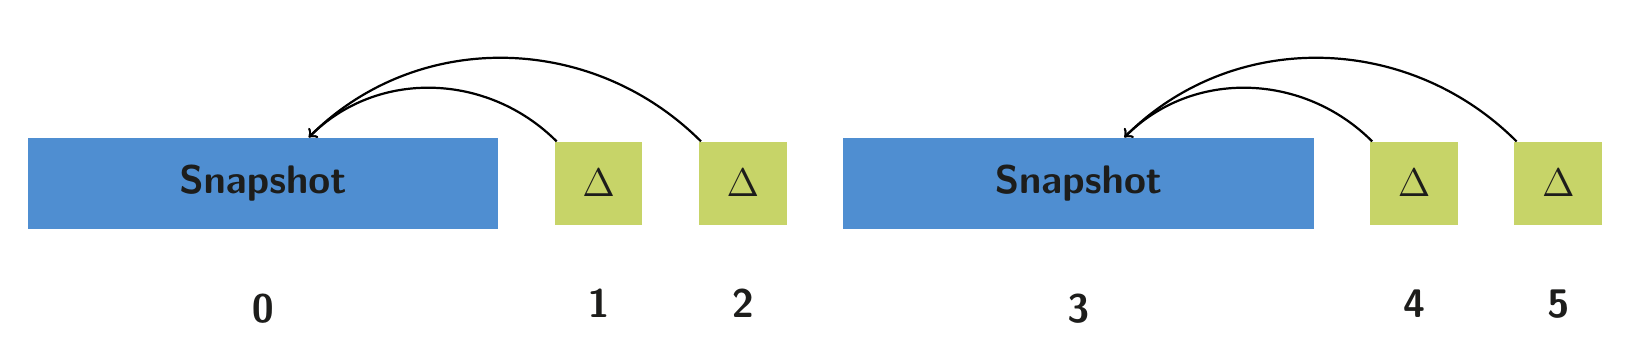
\begin{tikzpicture}[
    node distance = 2em, auto,
    font={\Large\itshape},
    base/.style={text=colortext,font={\Large\bfseries},inner sep=10pt,align=center,rectangle},
    txt/.style={text=colortext,font={\Large\bfseries},align=center},
    treenode/.style={base,thick,draw=colortext,text width=2em},
    relation/.style={text width=13em},
]

    % Nodes
    \node[base,fill=colorsnapshot,text width=15em] (snapshot) {Snapshot};
    \node[base,fill=colordelta,right=of snapshot]  (delta1)   {$\Delta$};
    \node[base,fill=colordelta,right=of delta1]    (delta2)   {$\Delta$};
    \node[base,fill=colorsnapshot,text width=15em,right=of delta2] (snapshot2) {Snapshot};
    \node[base,fill=colordelta,right=of snapshot2]    (delta4)   {$\Delta$};
    \node[base,fill=colordelta,right=of delta4]    (delta5)   {$\Delta$};
    
    % Text
    \node[txt,below=of snapshot]  (snaptxt) {0};
    \node[txt,below=of delta1]  (delta1txt) {1};
    \node[txt,below=of delta2]  (delta1txt) {2};
    \node[txt,below=of snapshot2] (snaptxt) {3};
    \node[txt,below=of delta4]              {4};
    \node[txt,below=of delta5]              {5};
    
    % Arrows
    \draw[->,thick](delta1) to [out=135,in=45] (snapshot);
    \draw[->,thick](delta2) to [out=135,in=45] (snapshot);
    \draw[->,thick](delta4) to [out=135,in=45] (snapshot2);
    \draw[->,thick](delta5) to [out=135,in=45] (snapshot2);

\end{tikzpicture}
\end{document}
